\documentclass{beamer}
\usecolortheme{dove}
\setbeamertemplate{navigation symbols}{}
\usepackage{amsmath,amssymb,amsfonts,amsthm, multicol, subfigure, color}
\usepackage{bm}
\usepackage{graphicx}
\usepackage{tabularx}
\usepackage{booktabs}
\usepackage{hyperref}
\usepackage{pdfpages}
\usepackage{xcolor}
\definecolor{seagreen}{RGB}{46, 139, 87}
\def\independenT#1#2{\mathrel{\rlap{$#1#2$}\mkern2mu{#1#2}}}
\newcommand\indep{\protect\mathpalette{\protect\independenT}{\perp}}
\def\log{\text{log}}
\newcommand\logit{\text{logit}}
\newcommand\iid{\stackrel{\text{iid}}{\sim}}
\newcommand\E{\text{E}}
\newcommand\V{\text{V}}
\renewcommand\P{\text{P}}
\newcommand{\Cov}{\text{Cov}}
\newcommand{\Cor}{\text{Cor}}
\newcommand\doop{\text{do}}


\usepackage{stackrel}
\usepackage{tikz}
\usetikzlibrary{arrows,shapes.arrows,positioning,shapes,patterns,calc}
\newcommand\slideref[1]{\vskip .1cm \tiny \textcolor{gray}{{#1}}}
\newcommand\red[1]{\color{red}#1}
\newcommand\blue[1]{\color{blue}#1}
\newcommand\gray[1]{\color{gray}#1}
\newcommand\seagreen[1]{\color{seagreen}#1}
\newcommand\purple[1]{\color{purple}#1}
\newcommand\orange[1]{\color{orange}#1}
\newcommand\black[1]{\color{black}#1}
\newcommand\white[1]{\color{white}#1}
\newcommand\teal[1]{\color{teal}#1}
\newcommand\magenta[1]{\color{magenta}#1}
\newcommand\Fuchsia[1]{\color{Fuchsia}#1}
\newcommand\BlueGreen[1]{\color{BlueGreen}#1}
\newcommand\bblue[1]{\textcolor{blue}{\textbf{#1}}}
\newcommand\bred[1]{\textcolor{red}{\textbf{#1}}}
\newcommand\bgray[1]{\textcolor{gray}{\textbf{#1}}}
\newcommand\bgreen[1]{\textcolor{seagreen}{\textbf{#1}}}
\newcommand\bref[2]{\href{#1}{\color{blue}{#2}}}
\colorlet{lightgray}{gray!40}
\pgfdeclarelayer{bg}    % declare background layer for tikz
\pgfsetlayers{bg,main} % order layers for tikz
\newcommand\mycite[1]{\begin{scriptsize}\textcolor{darkgray}{(#1)}\end{scriptsize}}
\newcommand{\tcframe}{\frame{
%\small{
\only<1|handout:0>{\tableofcontents}
\only<2|handout:1>{\tableofcontents[currentsection]}}
%}
}

\setbeamertemplate{footline}[frame number]

\setbeamertemplate{navigation symbols}{}

\addtobeamertemplate{footline}{
	\leavevmode%
	\hbox{%
		\begin{beamercolorbox}[wd=\paperwidth,ht=2.75ex,dp=.5ex,right,rightskip=1em]{mycolor}%
			\usebeamercolor[fg]{navigation symbols}\insertslidenavigationsymbol%
		\end{beamercolorbox}%
	}%
	\vskip0.5pt%
}{}




\usepackage[round]{natbib}
\bibliographystyle{humannat-mod}
\setbeamertemplate{enumerate items}[default]
\usepackage{mathtools}

\newcommand{\goalsframe}{\begin{frame}{Learning goals for today}
At the end of class, you will be able to:
\begin{enumerate}
\item Identify whether paths in a causal diagram are open or blocked given a conditioning set
\item Understand why conditioning on colliders differs from conditioning on non-colliders
\end{enumerate} \vskip .2in
\end{frame}}

\title{Conditional Independence in DAGs}
\author{INFO/STSCI/ILRST 3900: Causal Inference}
\date{19 Sep 2023}

\begin{document}


\begin{frame}[noframenumbering,plain]
  \titlepage
\end{frame}


\goalsframe


\begin{frame}{Logistics}
\begin{itemize}
\item Ch 6.4 of Hernan and Robins
\end{itemize}
\end{frame}



\begin{frame}
\frametitle{Causal Graphs}


\begin{itemize}
    \item Causal Directed Acyclic Graphs (DAG) help communicate modeling assumptions and implications \pause
    \item Check (marginal) independence by looking at paths in graph 
\end{itemize}

\end{frame}


\begin{frame}
\frametitle{Checking Marginal Independence}
\[A \rightarrow Z_1 \rightarrow Z_2 \leftarrow Z_3 \rightarrow Y\]


\vspace{2em}

\begin{itemize}

    \item Two types of nodes on a path:
\begin{itemize}
    \item Collider: $ \rightarrow Z \leftarrow $ \pause
    \item Non-colliders: $ \underbrace{\rightarrow Z \rightarrow}_{\text{mediator}}$ or $ \underbrace{\leftarrow Z \rightarrow}_{\text{common cause}} $\\
    \vspace{1em}

    \end{itemize}
    \pause
    \item Path is unblocked if it does \textbf{not} contain a collider \pause 
    \item Two variables are dependant if there is an unblocked path between them
\end{itemize}

\end{frame}

\begin{frame}
\frametitle{Exchangeability and DAGs}

\begin{itemize}
    \item (Marginal) Exchangeability: $Y^a \indep A$ \pause 
    \item \textbf{Causal path} path in which all arrows point from the treatment toward the outcome \pause
    \item Exchangeability holds if all unblocked paths are causal paths \pause  
     \item Conditional Exchangeability: $Y^a \indep A \mid L$ \pause 
     \item How do we tell if a path is open or blocked when conditioning on $L$?
\end{itemize}

\end{frame}




\begin{frame}
\frametitle{Open or blocked?}
How do we check if a path in the DAG is open or blocked when conditioning on a set of variables $L$?
    \[A \rightarrow Z_1 \rightarrow Z_2 \leftarrow Z_3 \rightarrow Y\]
\pause 
\begin{itemize}
    \item Check each node on the path
    \item If \textbf{any} node on the path is blocked, then the entire path is blocked
    \item If all nodes on the path are open, then the entire path is open
\end{itemize}

\pause

\vspace{2em}
Two variables are dependent conditional on $L$ if there is an unblocked path (when conditioning on $L$) between them  

\pause

\vspace{2em}
Conditional Exchangeability holds \textbf{given $L$} if all unblocked paths between $A$ and $Y$ are causal paths


\end{frame}



\begin{frame}
\frametitle{Common cause}


\vspace{2em}
\begin{figure}[t]
	\centering
	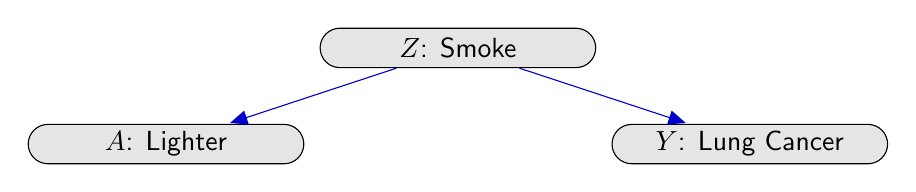
\begin{tikzpicture}[->,>=triangle 45,shorten >=1pt,
	auto, main node/.style={rounded rectangle,inner sep=0pt,fill=gray!20,draw,font=\sffamily,
		minimum width = 3.5cm, minimum height = .5cm}]

    \node[main node] (L) {$Z$: Smoke};
    \node[main node] (X) [below left = 1cm of L] {$A$: Lighter};
    \node[main node] (Y) [below right = 1cm of L] {$Y$: Lung Cancer};

	\path[color=black!20!blue,style={->}]
	(L) edge node {} (Y)
 	(L) edge node {} (X);

	\end{tikzpicture}

\end{figure}

\pause 
\vspace{2em}
If $Z$ has a causal effect on both $A$ and $Y$, the path is blocked when we condition on $Z$


\end{frame}

\begin{frame}
\frametitle{Mediation}


\vspace{2em}
\begin{figure}[t]
	\centering
	
\begin{tikzpicture}[->,>=triangle 45,shorten >=1pt,
	auto, main node/.style={rounded rectangle,inner sep=0pt,fill=gray!20,draw,font=\sffamily,
		minimum width = 3cm, minimum height = .5cm}]

    \node[main node] (X) {$A$: Sodium};
    \node[main node] (1) [right = .5cm of X] {$Z$: High Blood Pressure};
%    \node[main node] (2) [below = 1cm of 1] {Good Taste};
    \node[main node] (Y) [right = .5cm of 1] {$Y$: Heart Disease};
%\only<2>{\node[main node] (E) [below = .8cm of 1] {Email classmates};}

    \path[color=black!20!blue,style={->}]
	(X) edge node {} (1)
	(1) edge node {} (Y);
%\only<2>{\path[color=black!20!blue,style={->}]
%	(1) edge node {} (E);}
%	(X) edge node {} (Y)
%	(2) edge node {} (X)
%	(2) edge node {} (Y)	;
	
	\end{tikzpicture}
\end{figure}

\pause 
\vspace{2em}
If $A$ effects $Y$ through $Z$, the path is blocked when we condition on $Z$

\end{frame}




\begin{frame}
\frametitle{Types of paths}
\pause 
For non-colliders
\begin{itemize}
    \item Mediators: $ \rightarrow Z \rightarrow \quad$ or $\quad \leftarrow Z \leftarrow $
    \item Common causes: $ \leftarrow Z \rightarrow $
\end{itemize}
\pause 
\vspace{2em}
\begin{itemize}
    \item If $Z$ is in the conditioning set, then $Z$ is blocked \pause 
% \item If a descendant of $Z$ is in the conditioning set $L$, then $Z$ is partially blocked \pause 
    \item Otherwise, $Z$ is open 
\end{itemize}
\pause 

\[A \rightarrow Z_1 \rightarrow Z_2 \leftarrow Z_3 \rightarrow Y\]

\end{frame}





\begin{frame}
\frametitle{Collider}

\begin{figure}[t]
	\centering
	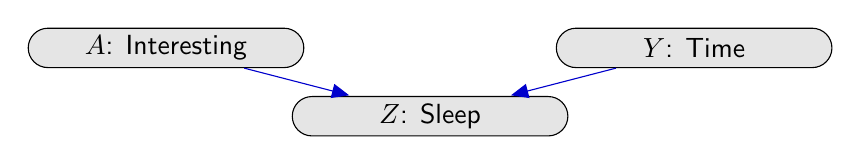
\begin{tikzpicture}[->,>=triangle 45,shorten >=1pt,
	auto, main node/.style={rounded rectangle,inner sep=0pt,fill=gray!20,draw,font=\sffamily,
		minimum width = 3.5cm, minimum height = .5cm}]

    \node[main node] (S) {$Z$: Sleep};
    \node[main node] (T) [above right = .5cm of S] {$Y$: Time};
    \node[main node] (I) [above left = .5cm of S] {$A$: Interesting};
	\path[color=black!20!blue,style={->}]
	(T) edge node {} (S)
	(I) edge node {} (S);

	\end{tikzpicture}

\end{figure}

\only<2>{
Mathematically, 
\[Z = X + Y \]
If we keep $Z$ fixed, but increase $X$, then to preserve the equation, $Y$ must decrease
}

\end{frame}

\begin{frame}
\frametitle{Collider}

\begin{figure}[t]
	\centering
	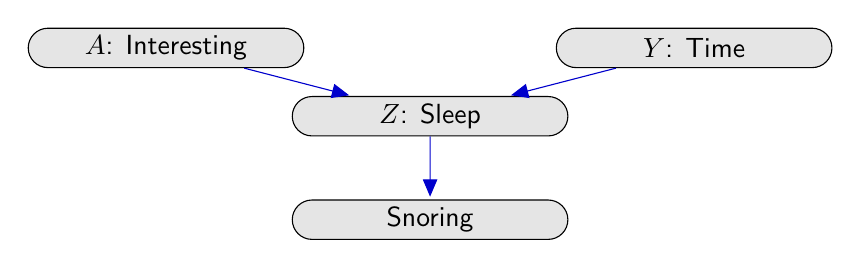
\begin{tikzpicture}[->,>=triangle 45,shorten >=1pt,
	auto, main node/.style={rounded rectangle,inner sep=0pt,fill=gray!20,draw,font=\sffamily,
		minimum width = 3.5cm, minimum height = .5cm}]

    \node[main node] (S) {$Z$: Sleep};
    \node[main node] (T) [above right = .5cm of S] {$Y$: Time};
    \node[main node] (I) [above left = .5cm of S] {$A$: Interesting};
    \node[main node] (E) [below = .8cm of S] {Snoring};

	\path[color=black!20!blue,style={->}]
	(T) edge node {} (S)
	(I) edge node {} (S)
	(S) edge node {} (E);

	\end{tikzpicture}

\end{figure}

\pause
\begin{itemize}
    \item If there is a causal path $X \rightarrow \ldots \rightarrow Z$, then $Z$ is a descendant of $X$  
\end{itemize}

\end{frame}




\begin{frame}
\frametitle{Colliders}
For Colliders $ \rightarrow Z \leftarrow $\pause 



\vspace{2em}

\begin{itemize}
    \item If $Z$ (or any descendant of $Z$) is in the conditioning set, then $Z$ is open
    \item Otherwise $Z$ is blocked
\end{itemize}
\pause 

    \[A \rightarrow Z_1 \rightarrow Z_2 \leftarrow Z_3 \rightarrow Y\]


\end{frame}


\begin{frame}
\frametitle{Open or blocked?}

How to check if a path is open or blocked:
\begin{enumerate}
    \item Traverse the path node by node \pause 
    \item If any node is blocked, the entire path is blocked
    \item If all nodes are open, then entire path is open
\end{enumerate}

\pause 
\vspace{2em}

How to check if a node is open or blocked:
\begin{itemize}
    \item If non-collider:
    \begin{itemize}
        \item Open if it is not in the conditioning set
        \item Blocked if it is in the conditioning set
    \end{itemize} \pause
    \item If collider:
    \begin{itemize}
        \item Open if it or any of its descendants are in the conditioning set
        \item Otherwise it is blocked
    \end{itemize} \pause
\end{itemize}

\end{frame}




\begin{frame}
\frametitle{Exercise}

\begin{figure}
\begin{tikzpicture}[x = \textwidth, y = .8\textheight]
\node (a) at (.5, .45) {$A$};
\node (u1) at (.25, .6) {$Z_1$};
\node (x) at (.4, .525) {$Z_2$};
\node (u2) at (.25, .45) {$Z_3$};
\node (y) at (.7, .45) {$Y$};
\draw[->, thick] (u1) to[out = 0, in = 135] (y);
\draw[->, thick] (u1) -- (x);
\draw[->, thick] (u2) -- (x);
\draw[->, thick] (u2) -- (a);
\draw[->, thick] (a) -- (y);
\end{tikzpicture}
\end{figure}

\begin{itemize}
    \item What are the paths from $A$ to $Y$?
    \item When conditioning on $L = \{Z_1\}$ are those paths open or blocked?
    \item When conditioning on $L = \{Z_2\}$ are those paths open or blocked?
    \item When conditioning $L = \{Z_1, Z_2\}$ are those paths open or blocked?
\end{itemize}

\end{frame}


\begin{frame}
\frametitle{Exercise}

\begin{figure}
\begin{tikzpicture}[x = \textwidth, y = .8\textheight]
\node (a) at (.25, .45) {$A$};
\node (b) at (.5, .45) {$Z_1$};
\node (d) at (.5, .25) {$Z_2$};
\node (g) at (.5, .65) {$Z_3$};
\node (y) at (.75, .45) {$Y$};
\draw[->, thick] (a) -- (b);
\draw[->, thick] (b) -- (y);
\draw[->, thick] (d) -- (y);
\draw[->, thick] (g) -- (b);
\draw[->, thick] (g) -- (y);
\draw[->, thick] (a) -- (d);

\end{tikzpicture}
\end{figure}

\begin{itemize}
    \item What are the paths from $A$ to $Y$?
    \item When conditioning on $L = \{Z_2\}$ are those paths open or blocked?
    \item When conditioning $L = \{Z_1, Z_2\}$ are those paths open or blocked?
\end{itemize}

\end{frame}




\goalsframe


\end{document}

